%!TEX root = ../thesis-summary.tex

\section{Implementation Details}
\label{section:appendix}

This Appendix includes detailed Figures, Listings and other resources that give
an expanded view of Pulsarcast's architecture and implementation.

\begin{figure}
  \centering
  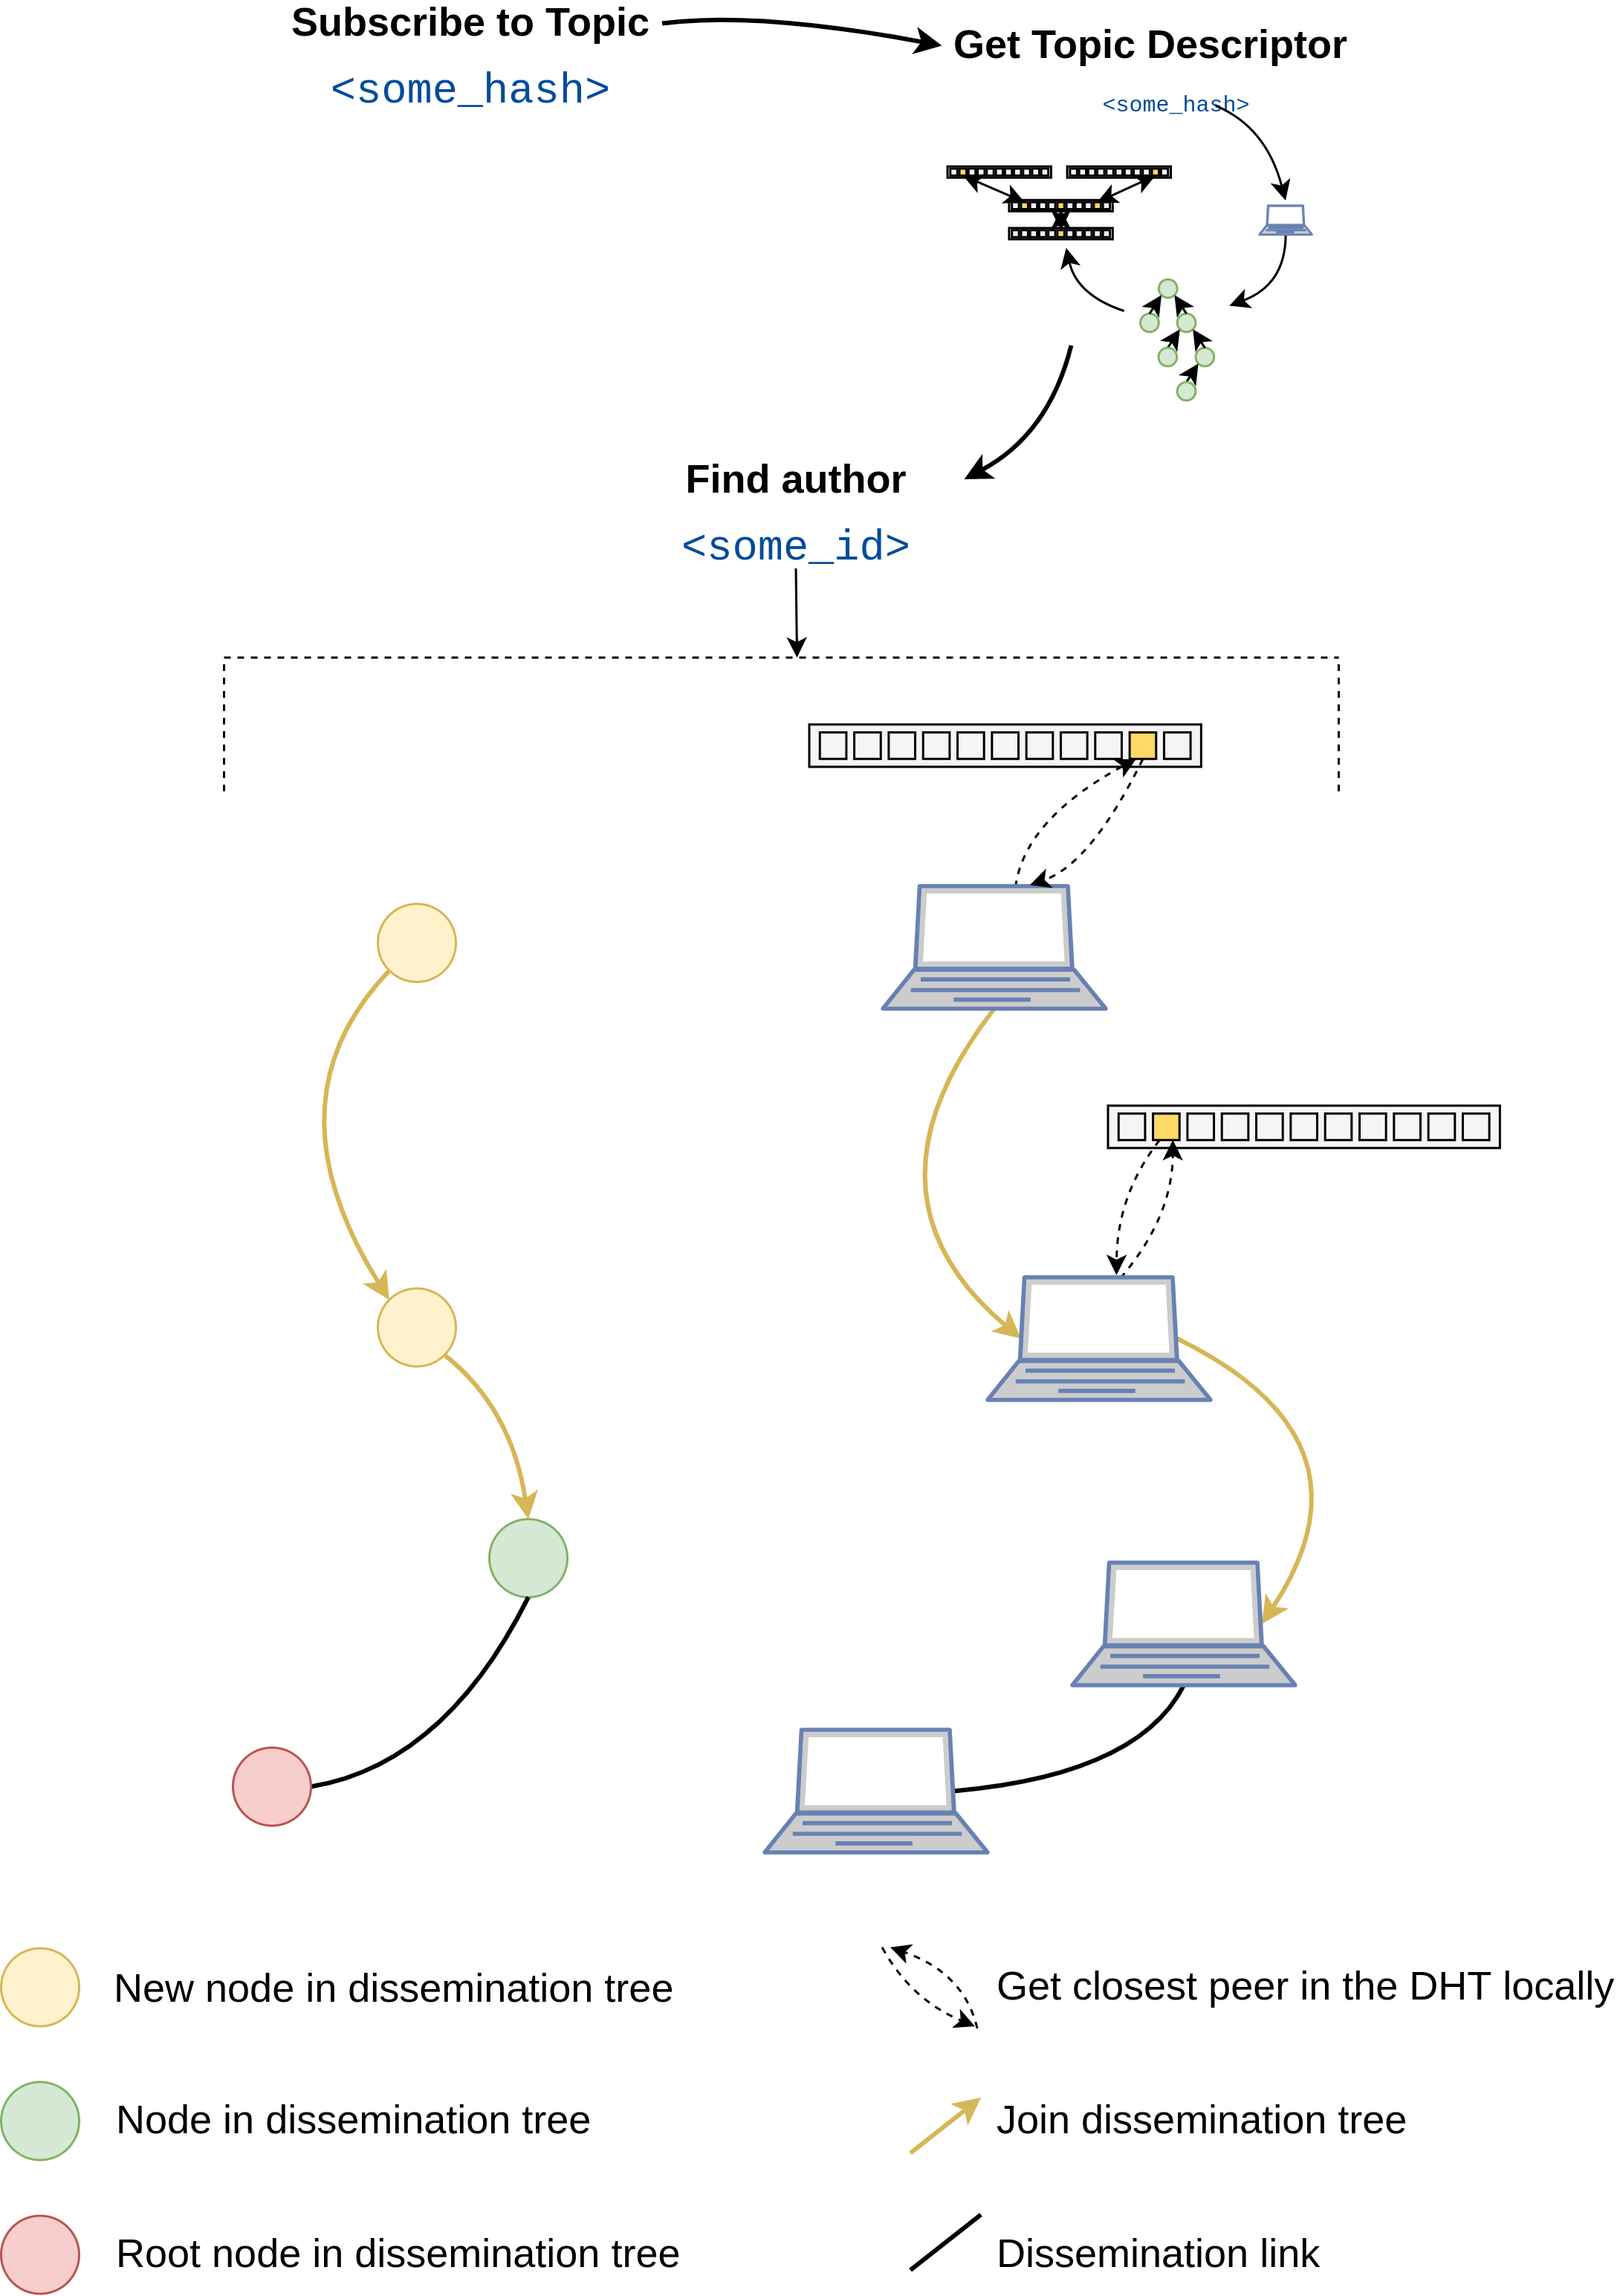
\includegraphics[width=0.4\textwidth]{../images/pulsarcast-subscription-flow.png}
  \caption{Overview of the flow for creating a new subscription}
  \label{fig:pulsarcast-subscription-flow}
\end{figure}

\begin{figure}
  \centering
  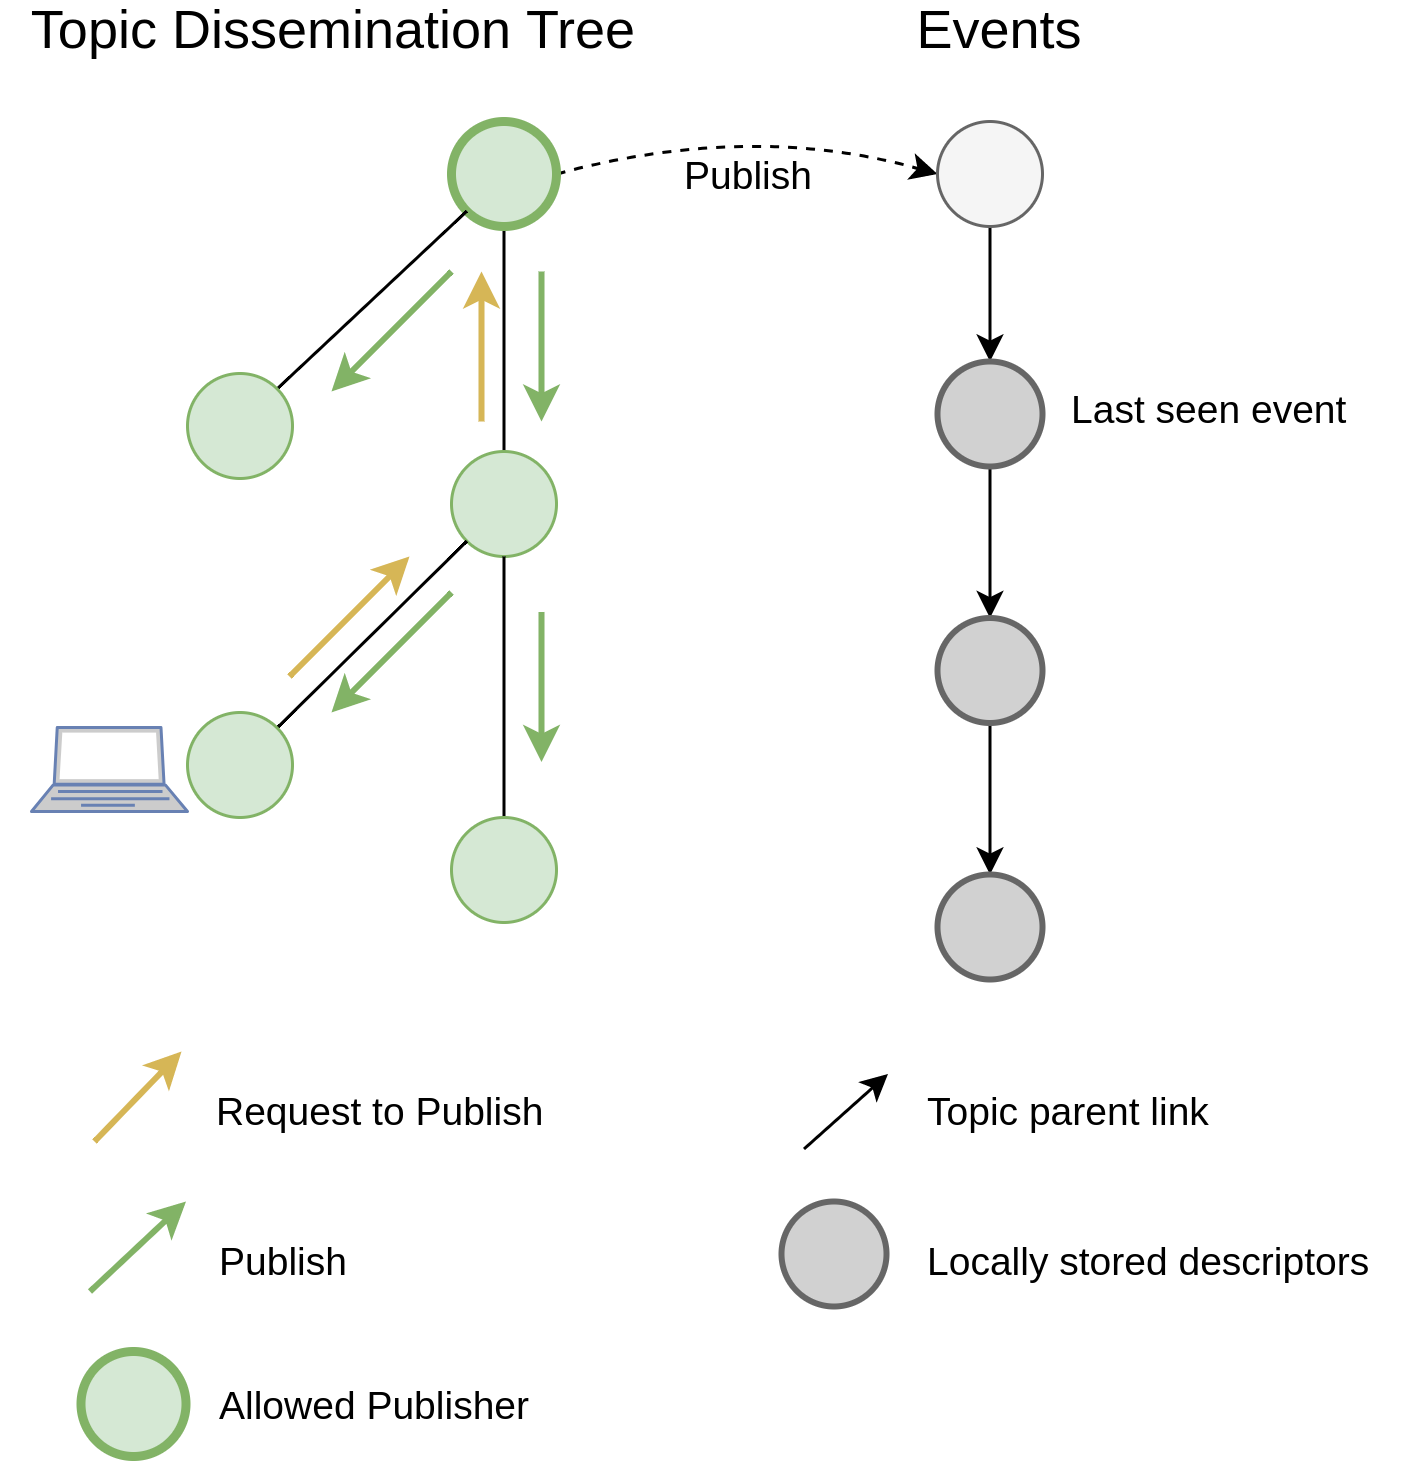
\includegraphics[width=0.3\textwidth]{../images/pulsarcast-publish-order-guarantee.png}
  \caption{Event dissemination mechanism for a topic with only the author allowed to publish, last seen event linking and request to publish allowed. This scenario provides order guarantee.}
  \label{fig:pulsarcast-publish-order-guarantee}
\end{figure}

\begin{figure}
  \centering
  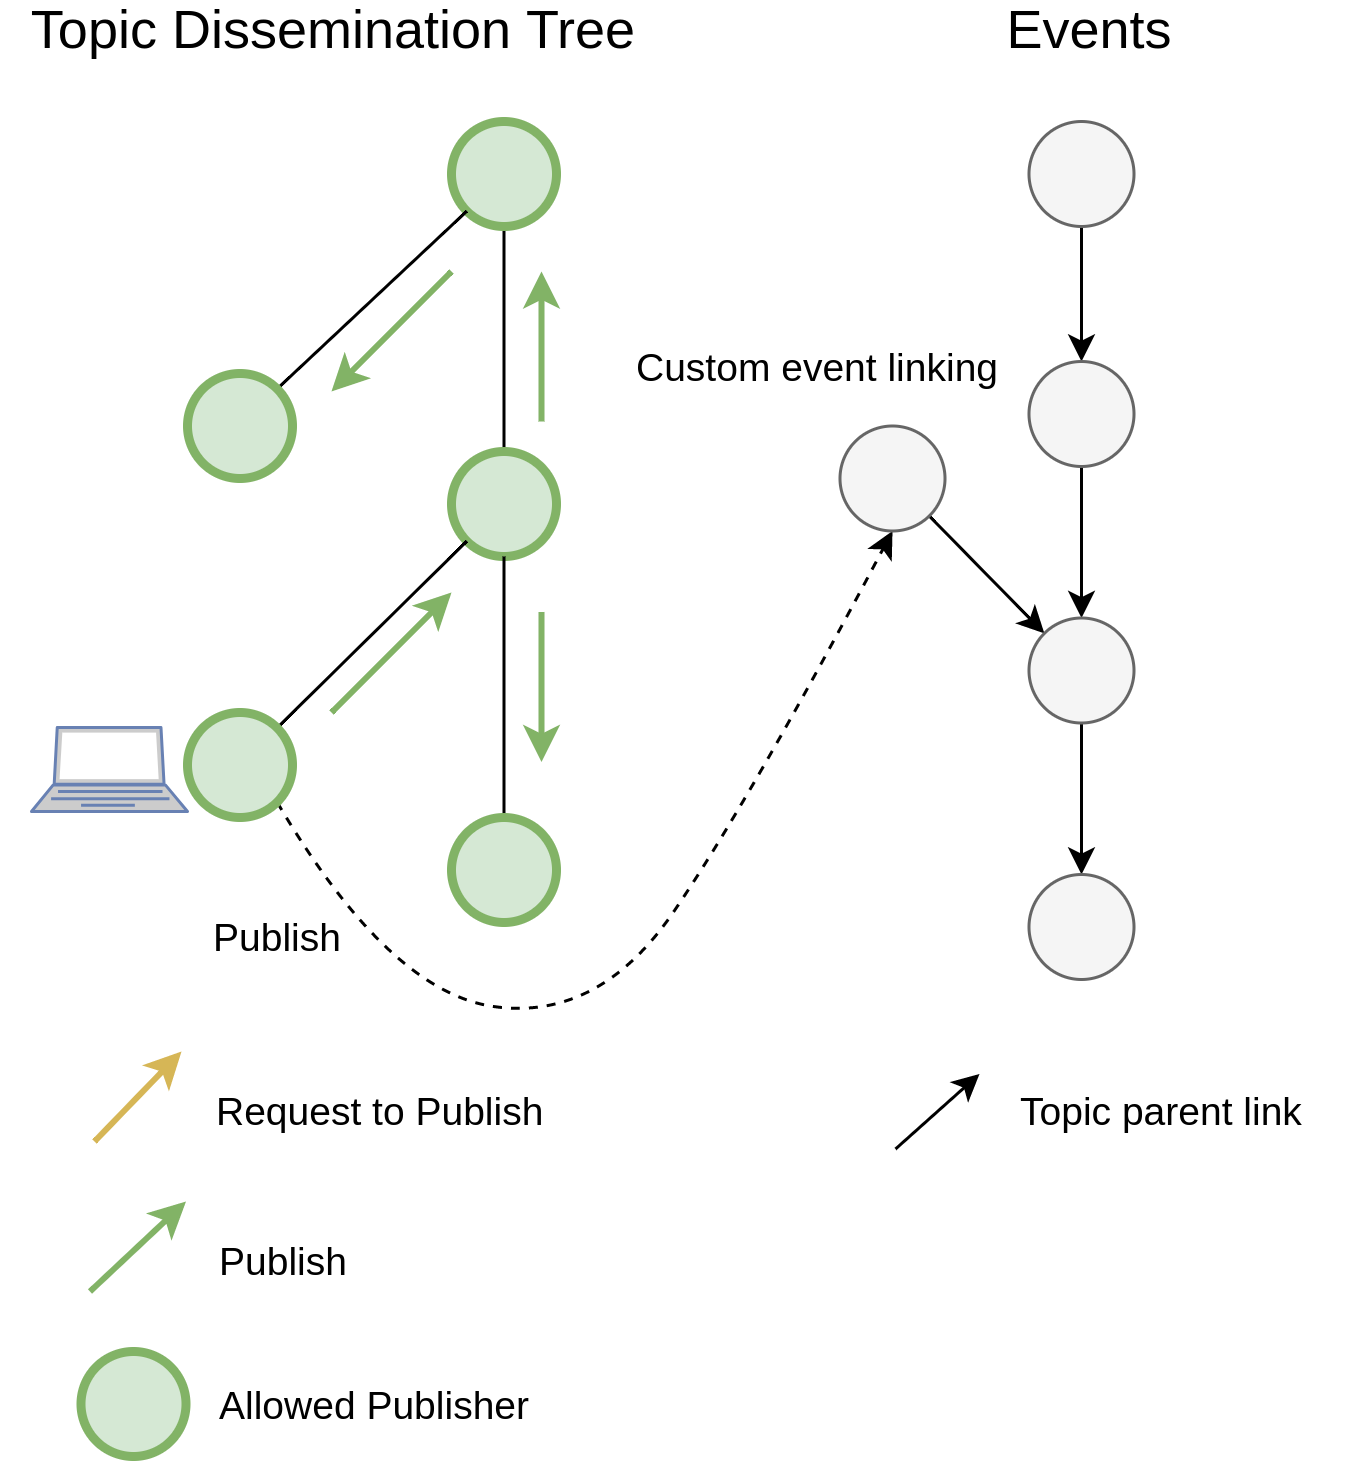
\includegraphics[width=0.3\textwidth]{../images/pulsarcast-publish-custom.png}
  \caption{Event dissemination mechanism for a topic with custom event linking and global publishers allowed}
  \label{fig:pulsarcast-publish-custom}
\end{figure}

\begin{lstlisting}[language=JavaScript, float=h, caption={Usage example of our Pulsarcast module},label={pulsarcast-usage-example}]
const Pulsarcast = require('pulsarcast')

// node is a libp2p Node
const pulsarcastNode = new Pulsarcast(node)

const pulsarcastNode.start((err) => {
  if (err) console.log('No!!!', err)
  
  pulsarcastNode.createTopic('fuuuuun', (err, cid, topicNode) => {
    if (err) console.log('No!!!', err)
    console.log('Our new topic \o/', topicNode)
    
    pulsarcastNode.on(cid.toBaseEncodedString(), (eventNode) => {
      console.log('event', eventNode)
    })
    
    pulsarcastNode.publish(cid.toBaseEncodedString(), new Buffer('super fun!'), (err, eventCID) => {
      if (err) console.log('No!!!', err)
      console.log('published', eventCID.toBaseEncodedString())
    })
  })
})
\end{lstlisting}

\section{Evaluation Details}
\label{ap:evaluation-details}

\subsection{Testbed}
\label{ap:sub:testbed}
As part of our implementation, we needed a way to test our Pulsarcast system.
However we had a set of specific requirements that made our choice of tools
harder. We needed something that fulfilled the following:

\begin{itemize}
  \item Easily deploy and test different versions of our module.
  \item Run tests not only on Pulsarcast but also on IPFS' own pub-sub
    implementation.
  \item Able to extract relevant usage metrics.
  \item Simulate network constraints such as latency.
  \item Able to run locally but easily scalable to a large network.
  \item Can be controlled from a central point, while being able to interact
    with specific nodes in the system.
  \item Easy to create scripts for, so that we could automate as much of our
    test suite as possible.
\end{itemize}

To achieve this we relied on containers, specifically
Docker~\footnote{\url{https://www.docker.com/products/container-runtime}}
containers, which we used to create a containerised version of our module. To
orchestrate our containerised application we used
Kubernetes~\footnote{\url{https://kubernetes.io/}}, an open source
orchestration platform based on Google's learnings on running containerised
workloads at scale~\footnote{\url{https://research.google/pubs/pub43438/}}, and
one of the most popular solutions in the field.

To aggregate, correlate and analyse metrics and logs we used
Elasticsearch~\footnote{\url{https://www.elastic.co/products/elasticsearch}},
Beats~\footnote{\url{https://www.elastic.co/products/beats}},
Logstash~\footnote{\url{https://www.elastic.co/products/logstash}} and
Kibana~\footnote{\url{https://www.elastic.co/products/kibana}}. In order to
simulate abnormal network conditions we relied on
Toxiproxy~\footnote{\url{http://toxiproxy.io}}, a TCP proxy that,
programatically through an HTTP API, allowed us to inject multiple kinds of
faults.

As we know it, Pulsarcast is just a module that applications can use to build
on top of. In order to test it we created a fork of JS
IPFS~\footnote{\url{https://github.com/jgantunes/js-ipfs}} where we integrated
Pulsarcast. This not only provided us with a command line interfaace (CLI) and
an HTTP API to interact with our system, but it also gave us direct access to
IPFS' own pub-sub module, Floodsub, to which we wanted to compare our module.

Figure \ref{fig:ipfs-testbed-and-metrics} provides an architectural overview of
our system. All of the projects and code we created for the testbed are
open
source~\footnote{\url{https://github.com/JGAntunes/helm-charts/tree/master/ipfs-testbed}}~\footnote{\url{https://github.com/JGAntunes/ipfs-testbed}}~\footnote{\url{https://github.com/JGAntunes/ipfs-testbed-cli}}.

\begin{figure}[!htb]
  \centering
  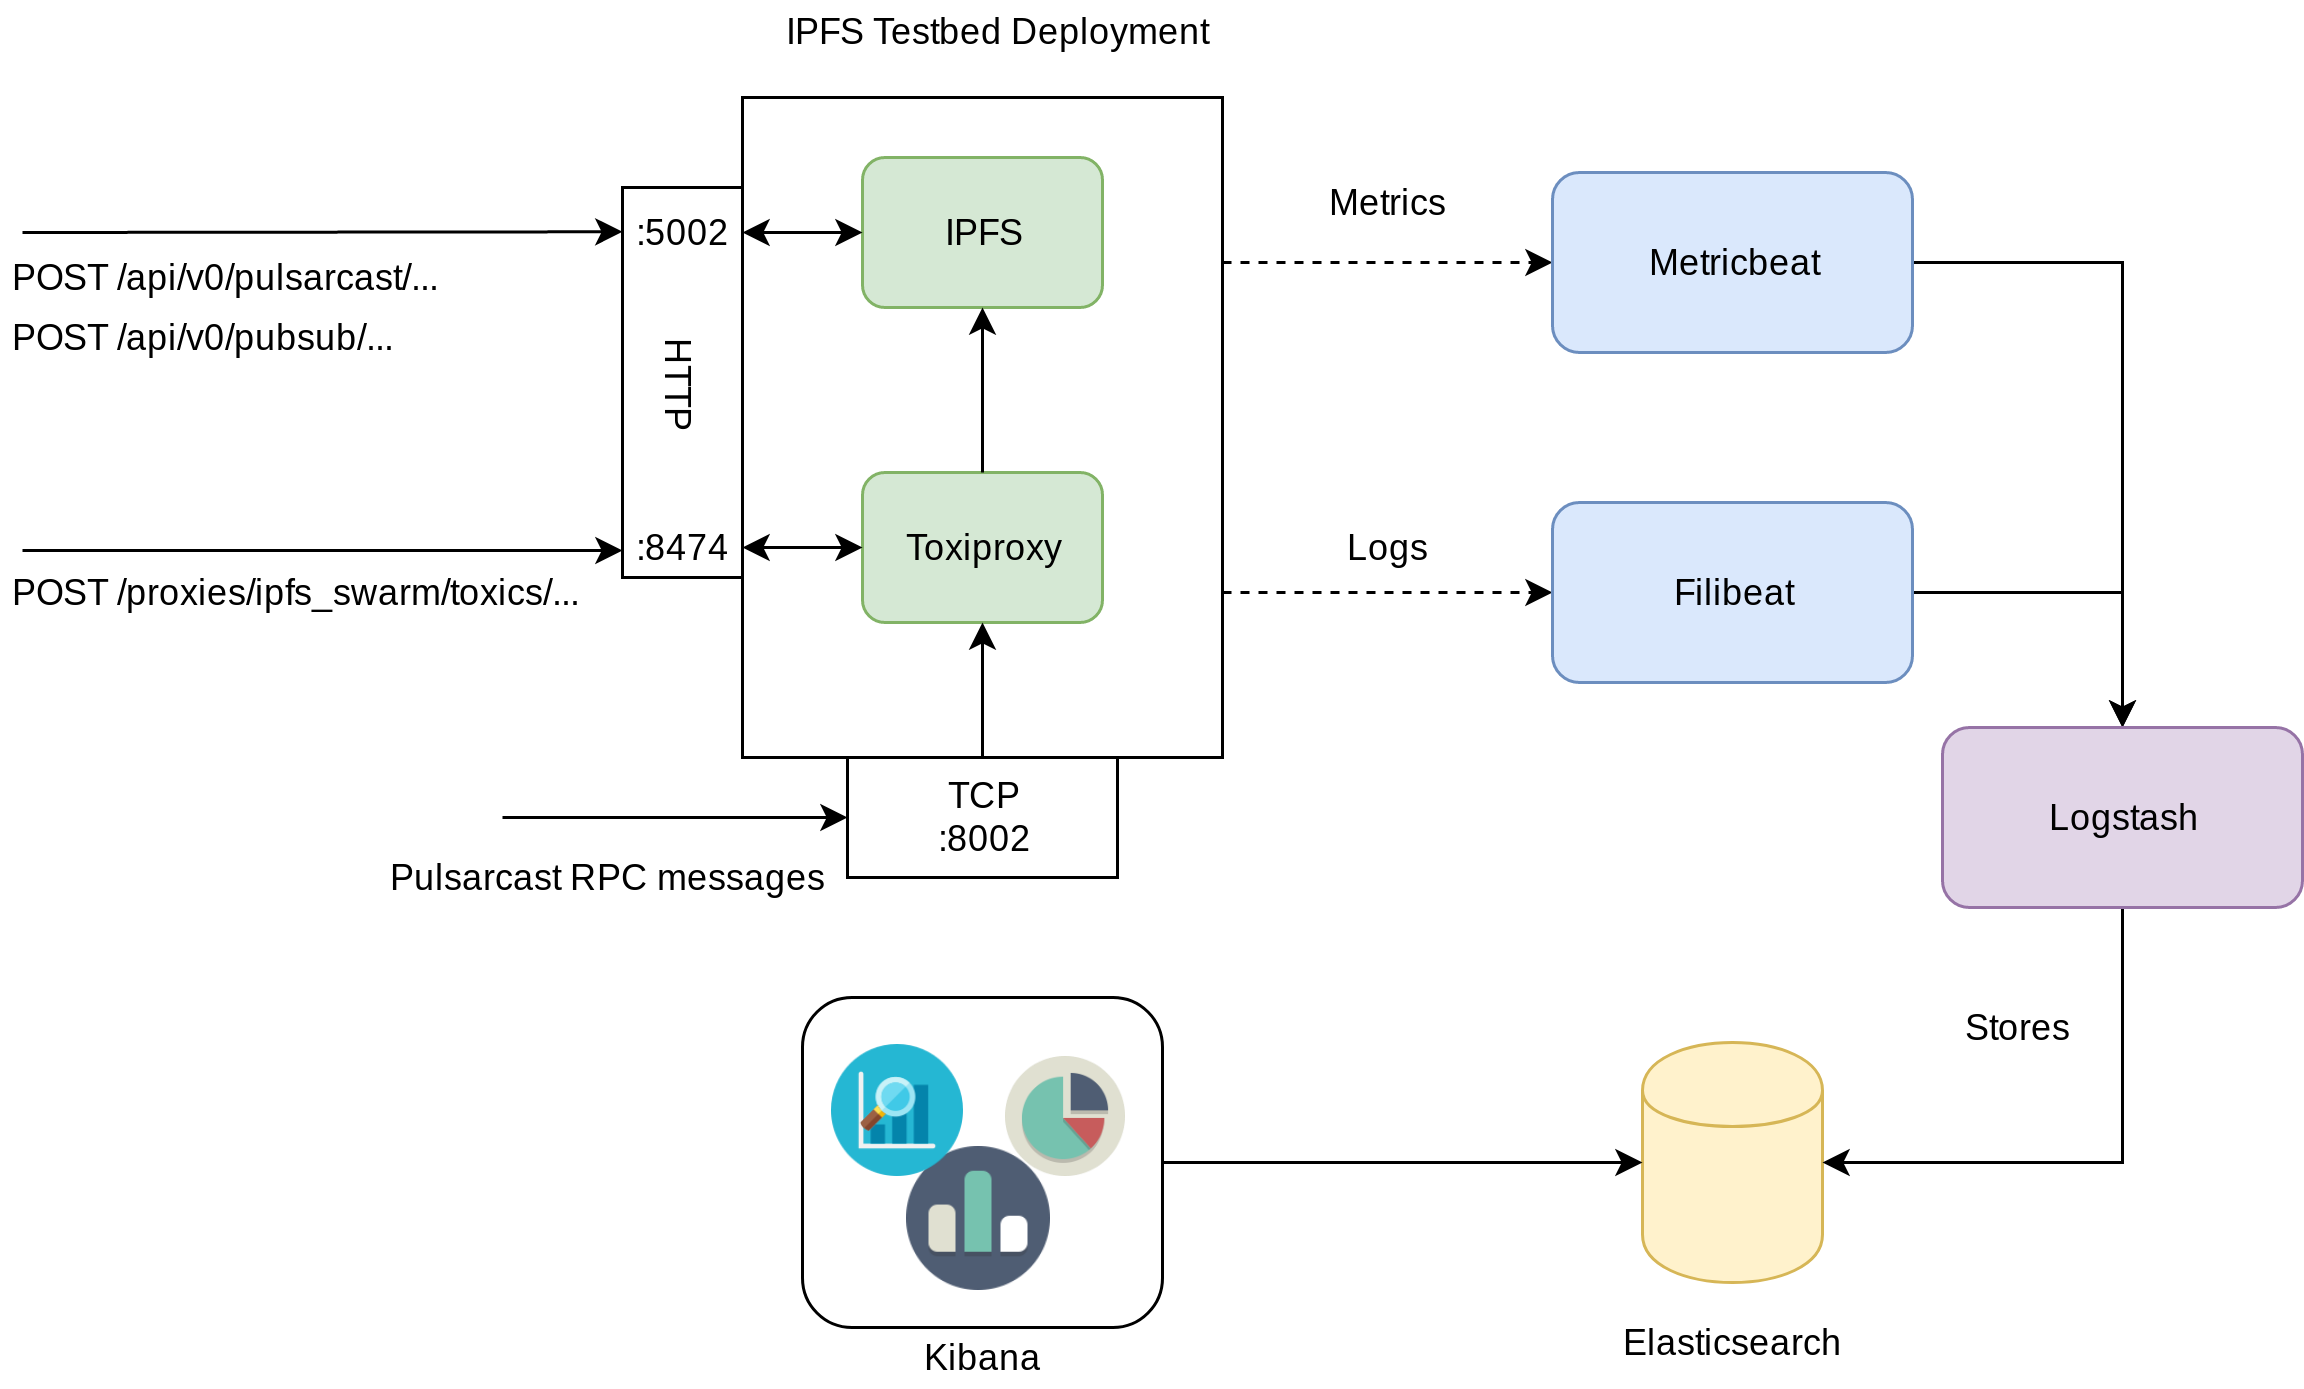
\includegraphics[width=0.45\textwidth]{../images/ipfs-testbed-and-metrics.png}
  \caption{Overview of our ipfs-testbed deployment and our metrics/logs
  pipeline}
  \label{fig:ipfs-testbed-and-metrics}
\end{figure}

\subsection{Detailed Results}
\label{ap:sub:detailed-results}

One aspect that we would like to highlight is the fact that we are not only
compressing months of data into a largely shorter timepsan, we are also
simulating interactions made by thousands of users into a much smaller set of
nodes (one hundred). All of this of course in an environment based on
virtualisation techniques and with a limited set of resources. This experiment
is essentially pushing the boundaries of what both systems would handle on a
real world scenario. Equally important to note is that, for Pulsarcast, every
event effectively published, is stored in the DHT. So, it is possible for any
application using Pulsarcast to resolve past or missing events from the event
tree. This is the cornerstone of Pulsarcast's eventual delivery guarantees,
hence why it is essential to look at the percentage of events effectively
published as well as the subscription coverage for these same events. Taking
those same numbers into consideration we can see a considerably high coverage
percentage, with the lowest being 62\% for the order guarantee test with
latency injected.

It is also important to highlight that, for all of the Pulsarcast executions we
have described, network and memory usage across the cluster always grew
linearly with the number of events received. Same for the RPC messages sent and
received, as we can see from Figure \ref{fig:graph-pulsarcast-rpc}

\begin{figure}[!htb]
  \centering
  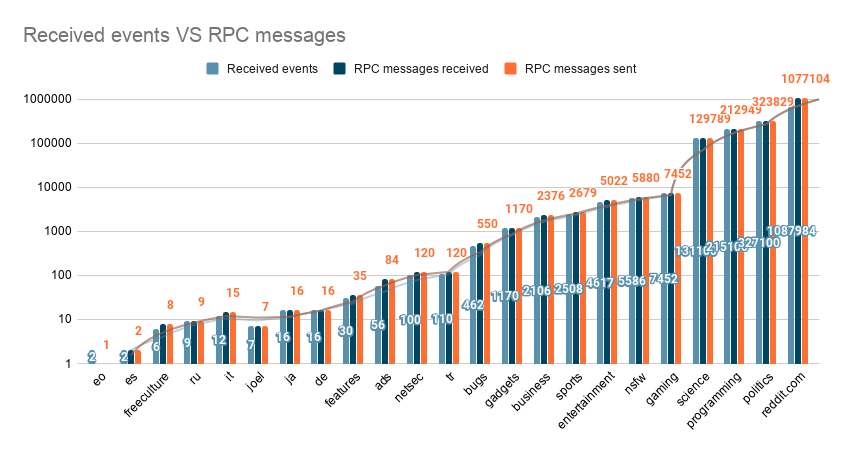
\includegraphics[width=0.4\textwidth]{../images/graph-pulsarcast-rpc.png}
  \caption{Pulsarcast without order guarantee - Comparison of events received and RPC injected in the system}
  \label{fig:graph-pulsarcast-rpc}
\end{figure}

\begin{figure}[!htb]
  \centering
  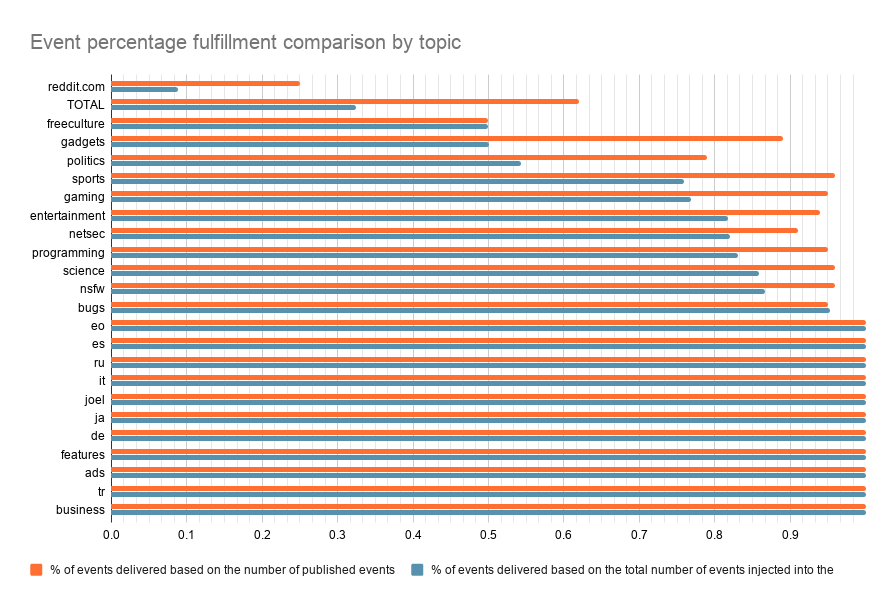
\includegraphics[width=0.4\textwidth]{../images/graph-pulsarcast-order-latency-event-percentage-fulfillment-comparison.png}
  \caption{Pulsarcast with order guarantee and latency - Comparison of percentage of events fulfilled by topic}
  \label{fig:graph-pulsarcast-order-latency-event-percentage-fulfillment-comparison}
\end{figure}

\begin{figure}[!htb]
  \centering
  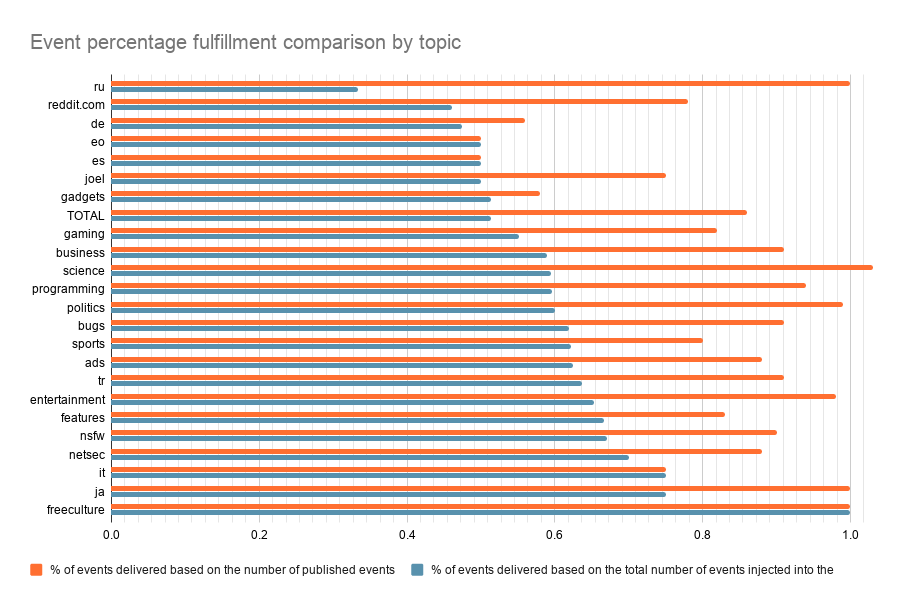
\includegraphics[width=0.4\textwidth]{../images/graph-pulsarcast-latency-event-percentage-fulfillment-comparison.png}
  \caption{Pulsarcast without order guarantee and latency - Comparison of percentage of events fulfilled by topic}
  \label{fig:graph-pulsarcast-latency-event-percentage-fulfillment-comparison}
\end{figure}
